\documentclass[boxes]{homework}

% This is a slightly-more-than-minimal document that uses the homework class.
% See the README at http://git.io/vZWL0 for complete documentation.

\name{傅申 PB20000051}        % Replace (Your Name) with your name.
\term{2022 秋}     % Replace (Current Term) with the current term.
\course{算法基础}    % Replace (Course Name) with the course name.
\hwnum{6}          % Replace (Number) with the number of the homework.
\hwname{作业}
\problemname{}
\solutionname{解:}

% Load any other packages you need here.
\usepackage[
    a4paper,
    top = 2.54cm,
    bottom = 2.54cm,
    left = 1.91cm,
    right = 1.91cm,
    includeheadfoot
]{geometry}
\fancyfootoffset{0pt} % make fancyhdr work properly
\usepackage{ctex}
\usepackage{tikz}
\tikzset{
    node/.style={circle, draw, inner sep=1pt, text centered},
    leaf/.style={rectangle, draw, rounded corners=2pt, inner sep=2pt, text centered},
    level/.style={sibling distance=4cm/#1, level distance=1cm}
}

\begin{document}
%%%% Problem 15.3-3 %%%%
\problemchap{15}
\problempart{3}
\problemnumber{3}
\begin{problem}
考虑矩阵链乘法问题的一个变形: 目标改为最大化举证序列括号化方案的标量乘法运算次
数, 而非最小化. 此问题具有最优子结构性质吗?
\end{problem}
\begin{solution}
    此问题仍具有最优子结构性质. 不妨假设 $A_{i}A_{i+1}\cdots A_{j}$ 的最优解在
    $A_{k}$ 和 $A_{k+1}$ 之间划分, 若 $A_{i}\cdots A_{k}$ 或
    $A_{k+1}\cdots A_{j}$ 没有采用它的最优解, 则将它的最优解代入原来
    $A_{i}\cdots A_{j}$ 的 ``最优解'' 中, 得到的运算次数比原来更高, 显然与假设的
    ``最优'' 性质矛盾, 故此问题的最优解包含其子问题的最优解, 也就是具有最优子结
    构性质.
\end{solution}

%%%% Problem 15.3-4 %%%%
\problemnumber{4}
\begin{problem}
如前所述, 使用动态规划方法, 我们首先求解子问题, 然后选择哪些子问题用来构造原问题
的最优解. Capulet 教授认为, 我们不必为了求原问题的最优解而总是求解出所有子问题.
她建议, 在求矩阵链乘法问题的最优解时, 我们总是可以在求解子问题\textit{之前}选定
$A_{i}A_{i+1}\cdots A_{j}$ 的划分位置 $A_{k}$ (选定的 $k$ 使得
$p_{i-1}p_{k}p_{j}$ 最小). 请找出一个反例, 证明这个方法可能生成次优解.
\end{problem}
\begin{solution}
    假设有 3 个矩阵 $A_{1}$, $A_{2}$, $A_{3}$, 对应的规模依次为 $p_{0} = 1000$,
    $p_{1} = 100$, $p_{2} = 10$, $p_{3} = 1$. 使用 Capulet 教授的方法, 选定的划
    分位置为 $k = 2$, 对应的括号化方案为
    $\left( \left( A_{1}A_{2}\right)A_{3}\right)$, 需要进行的标量乘法次数为
    $1000 \times 100 \times 10 + 1000 \times 10 \times 1 = 1010000$. 而最优括号
    化方案为 $\left( A_{1}\left( A_{2}A_{3}\right)\right)$, 需要进行的标量乘法次
    数为 $100 \times 10 \times 1 + 1000 \times 100 \times 1 = 101000 < 1010000$.
    因此 Capulet 的方法可能生成次优解.
\end{solution}


%%%% Problem 15.4-4 %%%%
\problempart{4}
\problemnumber{4}
\begin{problem}
说明如何只使用表 $c$ 中的 $2 \times \min (m, n)$ 个表项及 $O(1)$ 的额外空间来计
算 LCS 的长度. 然后说明如何只用 $\min(m, n)$ 个表项及 $O(1)$ 的额外空间完成相同
的工作.
\end{problem}
\begin{solution}
    因为计算表 $c$ 的某一行只需要其上一行的数据, 因此可以在完全计算完一行后就将
    上一行丢弃, 这样只需要表 $c$ 中两行的表项 (即 $2 \times \min(m,n)$) 及
    $O(1)$ 的额外空间.

    更进一步, 因为计算 $c[i, j]$ 只需要知道 $c[i - 1, j - 1]$, $c[i, j - 1]$,
    $c[i - 1, j]$, 所以实际上只需要一个临时变量存储 $c[i - 1, j - 1]$ 即可在 $c$
    的一行空间完成计算, 只需要重复地在这一行中从左往右依次更新表项值: 在更新这一
    行的第 $j$ 个表项前, 第 $j - 1$ 个表项的值就是 $c[i, j - 1]$, 第 $j$ 个表项
    中存储着 $c[i - 1, j]$, 临时变量中存储着 $c[i - 1, j - 1]$, 根据它们计算出
    $c[i, j]$, 然后将第 $j$ 个表项值存入临时变量, 再用 $c[i, j]$ 存入第 $j$ 个
    表项完成更新. 这样就能只用 $\min(m, n)$ 个表项及 $O(1)$ 的额外空间.
\end{solution}

%%%% Problem 15.5-2 %%%%
\problempart{5}
\problemnumber{2}
\begin{problem}
若 7 个关键字的概率如下所示, 求其最优二叉搜索树的结构和代价.
\begin{center}
    \begin{tabular}{c|cccccccc}
        \hline
        $i$     & 0    & 1    & 2    & 3    & 4    & 5    & 6    & 7    \\ \hline
        $p_{i}$ &      & 0.04 & 0.06 & 0.08 & 0.02 & 0.10 & 0.12 & 0.14 \\ \hline
        $q_{i}$ & 0.06 & 0.06 & 0.06 & 0.06 & 0.05 & 0.05 & 0.05 & 0.05 \\ \hline
    \end{tabular}
\end{center}
\end{problem}
\begin{solution}
    最优二叉搜索树的代价为 3.12, 结构如下
    \begin{center}
        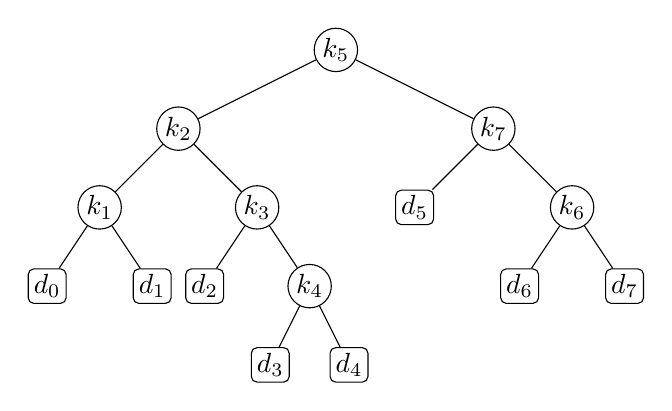
\begin{tikzpicture}
            \node[node] {$k_{5}$}
            child {
                    node[node] {$k_{2}$}
                    child {
                            node[node] {$k_{1}$}
                            child { node[leaf] {$d_{0}$} }
                            child { node[leaf] {$d_{1}$} }
                        }
                    child {
                            node[node] {$k_{3}$}
                            child { node[leaf] {$d_{2}$} }
                            child {
                                    node[node] {$k_{4}$}
                                    child { node[leaf] {$d_{3}$} }
                                    child { node[leaf] {$d_{4}$} }
                                }
                        }
                }
            child {
                    node[node] {$k_{7}$}
                    child { node[leaf] {$d_{5}$} }
                    child {
                            node[node] {$k_{6}$}
                            child { node[leaf] {$d_{6}$} }
                            child { node[leaf] {$d_{7}$} }
                        }
                };
        \end{tikzpicture}
    \end{center}
\end{solution}


%%%% Problem 16.1-3 %%%%
\problemchap{16}
\problempart{1}
\problemnumber{3}
\begin{problem}
对于活动选择问题, 并不是所有贪心方法都能得到最大兼容活动子集. 请举例说明, 在剩余
兼容活动中选择持续时间最短者不能得到最大集. 类似地, 说明在剩余兼容活动中选择与其
他剩余活动重叠最少者, 以及选择最早开始者均不能得到最优解.
\end{problem}
\begin{solution}
    考虑这样一个活动集合 $\{[1, 4), [3, 5), [4, 7)\}$, 选择持续时间最短者得到的
    子集为 $\{a_2\}$, 而最大兼容子集为 $\{a_1, a_3\}$, 没有得到最优解.

    考虑这样一个活动集合 $\{[1, 3), [2, 4), [2, 4), [2, 4), [3, 5), [4, 6),
        [5, 7), [6, 8), [6, 8), [6, 8), [7, 9)\}$, 选择与其他剩余活动重叠最少者
    会首先选择 $a_6 = [4, 6)$, 导致无法再选择 $a_5 = [3, 5)$ 和 $a_7 = [5, 7)$,
    而唯一的最大兼容子集为 $\{a_1 = [1, 3), a_5, a_7, a_{11} = [7, 9)\}$, 故无法
    得到最优解.

    考虑这样一个活动集合 $\{[1, 8), [2, 4), [4, 7)\}$, 选择开始最早者得到的子集
    为 $\{a_1\}$, 而最大兼容子集为 $\{a_2, a_3\}$, 没有得到最优解.
\end{solution}

\end{document}
